\subsubsection{Persistence Layer}

\begin{figure}[H]
    \centering
    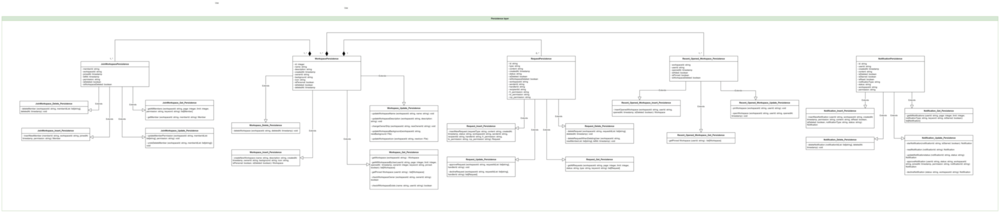
\includegraphics[ width = \linewidth]{Content/Phân tích và thiết kế hệ thống/documents/Sơ đồ lớp/images/Persistence layer/persistenceLayer.png}
    \vspace{0.5cm}
    \caption{Persistence Layer}
    \label{fig:Persistence Layer}
\end{figure}
Tầng Persistence sẽ nhận dữ liệu, yêu cầu từ tầng Business để thực hiện các thao tác tương tác với cơ sở dữ liệu, sau đó trả về kết quả cho tầng Business.

\begin{figure}[H]
    \centering
    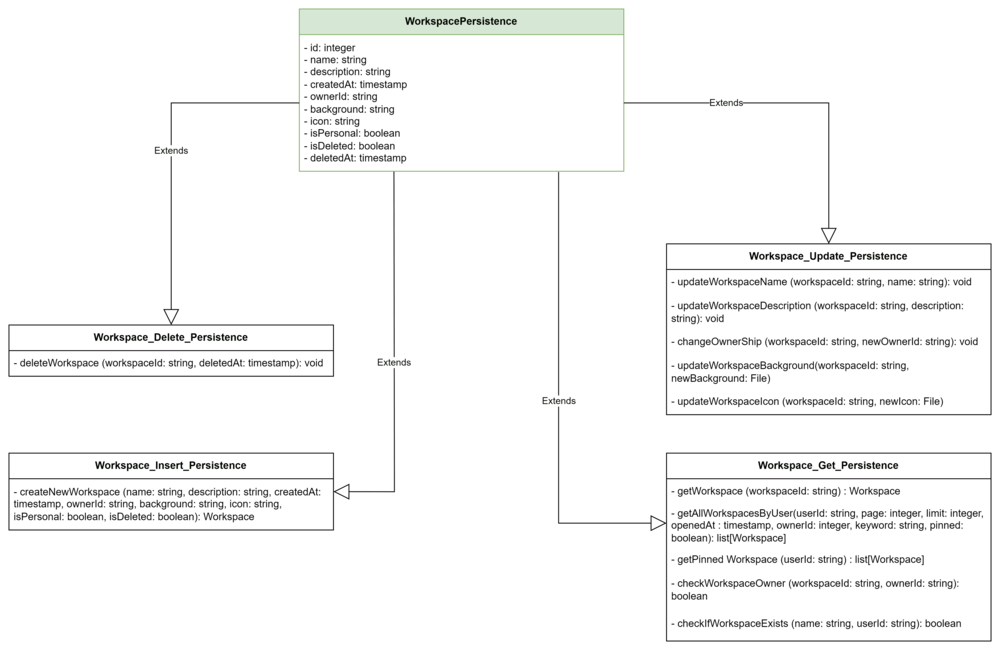
\includegraphics[ width = \linewidth]{Content/Phân tích và thiết kế hệ thống/documents/Sơ đồ lớp/images/Persistence layer/workspacePersistence.png}
    \vspace{0.5cm}
    \caption{Workspace Persistence}
    \label{fig:Workspace Persistence}
\end{figure}
\par
Class WorkspacePersistence sẽ chịu trách nhiệm thao tác với cơ sở dữ liệu 
liên quan đến bảng Workspace. Class này sẽ thừa kế các class khác như:
Workspace\_Get\_Persistence, Workspace\_Delete\_Persistence, Workspace\_Update\_Persistence.
Những class này sẽ thực hiện các chức năng tương ứng với tên của chúng.
\begin{figure}[H]
    \centering
    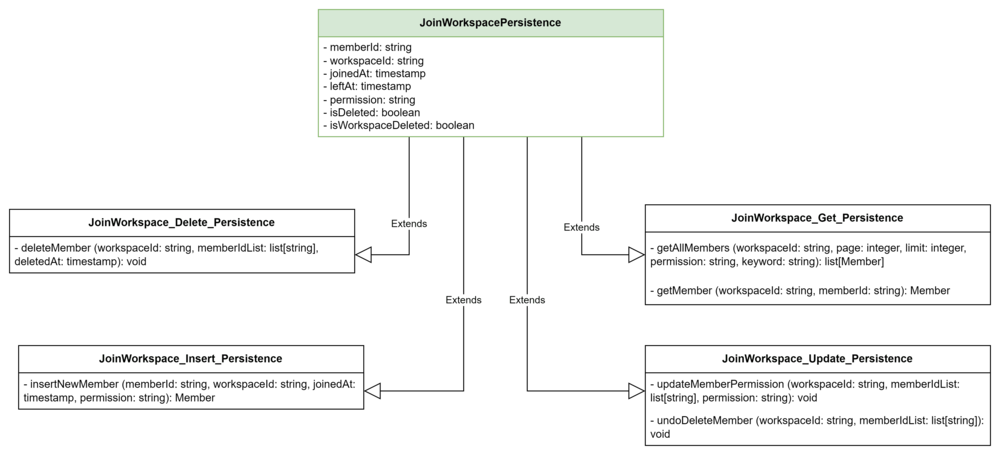
\includegraphics[ width = \linewidth]{Content/Phân tích và thiết kế hệ thống/documents/Sơ đồ lớp/images/Persistence layer/joinWorkspacePersistence.png}
    \vspace{0.5cm}
    \caption{Join Workspace Persistence}
    \label{fig:Join Workspace Persistence}
\end{figure}
\par
Class Join\_Workspace\_Persistence sẽ chịu trách nhiệm thao tác với cơ sở dữ liệu
liên quan đến bảng Join\_Workspace. Class này sẽ thừa kế các class khác như:
Join\_Workspace\_Get\_Persistence, Join\_Workspace\_Delete\_Persistence, Join\_Workspace\_Update\_Persistence.
\begin{figure}[H]
    \centering
    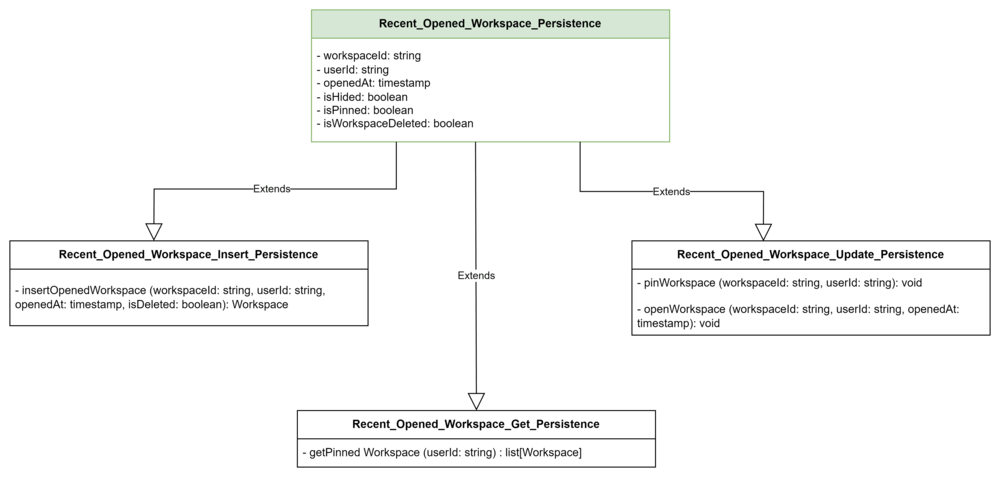
\includegraphics[ width = \linewidth]{Content/Phân tích và thiết kế hệ thống/documents/Sơ đồ lớp/images/Persistence layer/recentOpenedWorkspacePersistence.png}
    \vspace{0.5cm}
    \caption{Recent Opened Workspace Persistence}
    \label{fig:Recent Opened Workspace Persistence}
\end{figure}
\par
Class Recent\_Opened\_Workspace\_Persistence sẽ chịu trách nhiệm thao tác với cơ sở dữ liệu
liên quan đến bảng Recent\_Opened\_Workspace. Class này sẽ thừa kế các class khác như:
Recent\_Opened\_Workspace\_Get\_Persistence, Recent\_Opened\_Workspace\_Update\_Persistence.
\begin{figure}[H]
    \centering
    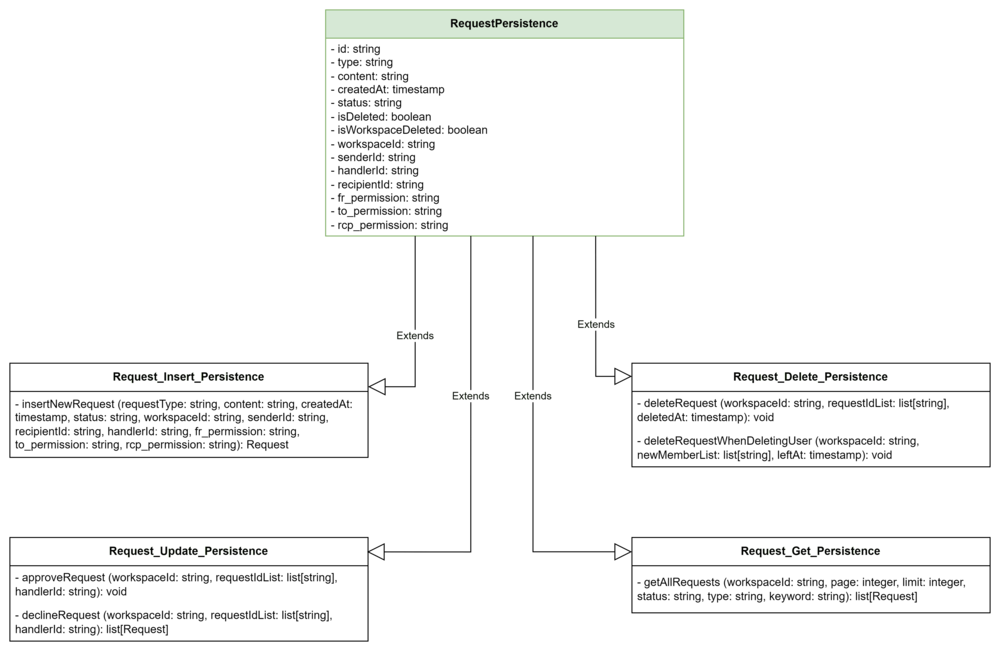
\includegraphics[ width = \linewidth]{Content/Phân tích và thiết kế hệ thống/documents/Sơ đồ lớp/images/Persistence layer/requestPersistence.png}
    \vspace{0.5cm}
    \caption{Request Persistence}
    \label{fig:Request Persistence}
\end{figure}
\par
Class Request\_Persistence sẽ chịu trách nhiệm thao tác với cơ sở dữ liệu
liên quan đến bảng Request. Class này sẽ thừa kế các class khác như:
Request\_Get\_Persistence, Request\_Delete\_Persistence, Request\_Update\_Persistence, Request\_Insert\_Persistence.
\begin{figure}[H]
    \centering
    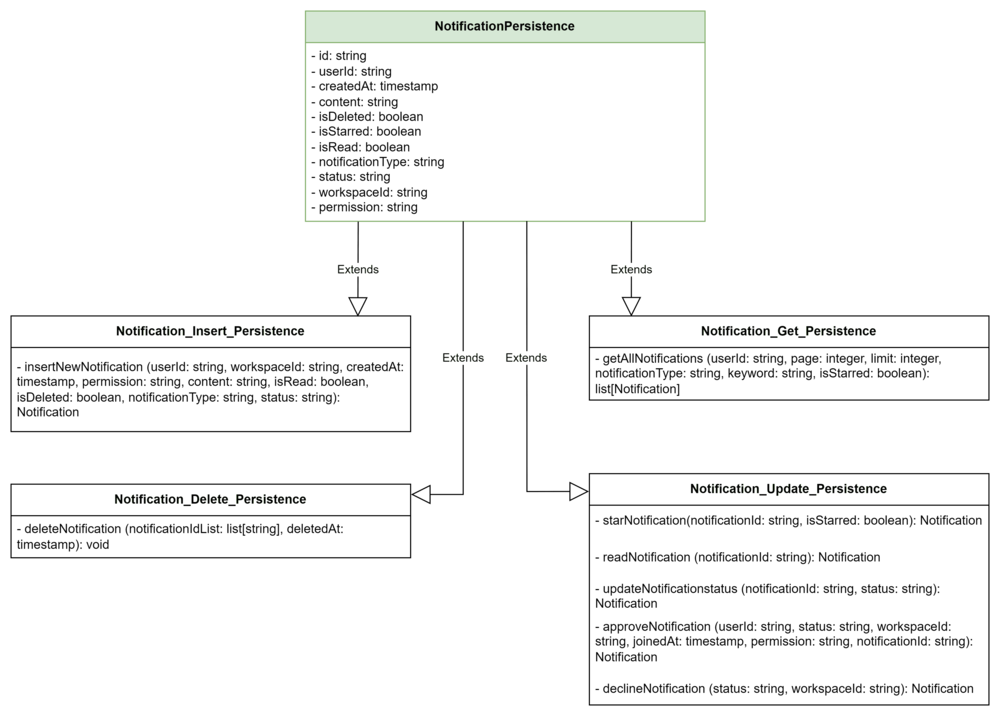
\includegraphics[ width = \linewidth]{Content/Phân tích và thiết kế hệ thống/documents/Sơ đồ lớp/images/Persistence layer/notificationPersistence.png}
    \vspace{0.5cm}
    \caption{Notification Persistence}
    \label{fig:Notification Persistence}
\end{figure}
\par
Class Notification\_Persistence sẽ chịu trách nhiệm thao tác với cơ sở dữ liệu
liên quan đến bảng Notification. Class này sẽ thừa kế các class khác như:
Notification\_Get\_Persistence, Notification\_Delete\_Persistence, Notification\_Update\_Persistence, Notification\_Insert\_Persistence.